\section{Aufbau der Spielarchitektur}

\subsection{Überblick}

Slick2D stellt Techniken zur Umsetzung eines zustandsbasierten Spieles zur Verfügung.
In Abbildung \ref{fig:spielarchitektur:states} werden die Zustände des Spiels und ihre Reihenfolge gezeigt.
Ein Spiel startet im \textit{MainMenuState}.
Hier kann der Spieler das Spiel entweder direkt beenden oder in den \textit{LevelMenuState} wechseln.
Der \textit{LevelMenuState} bietet eine Auswahl aller zur Verfügung stehenden Levels an, welche dann im \textit{PlayingState} gespielt werden können.
Während des Spiels kann das Spiel durch Wechsel in den \textit{PausMenuState} pausiert werden.
Nach erfolgreichem oder nicht erfolgreichem Abschluss eines Levels bietet der \textit{GameFinishState} die Möglichkeit das Level zu wechseln, das Level erneut zu spielen oder das Spiel zu beenden.

\begin{figure}[]
\centering
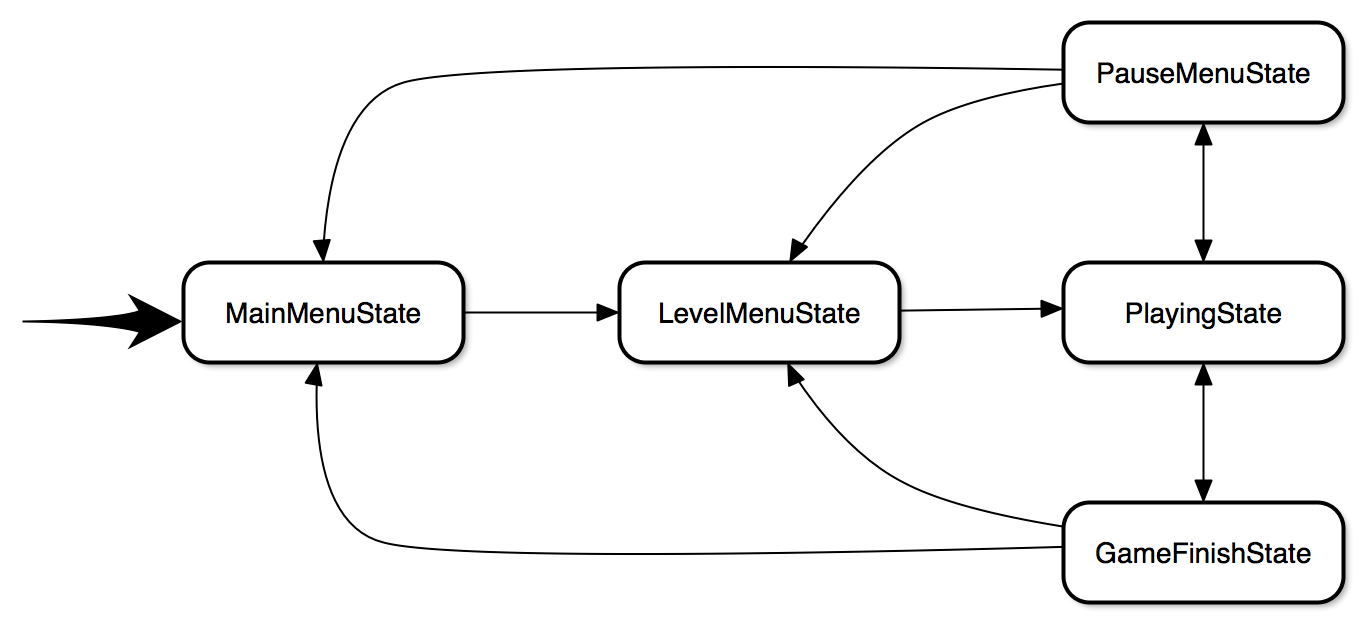
\includegraphics[width=3in]{img/05_states.png}
\caption{Übersicht der Zustände des Spiels}
\label{fig:spielarchitektur:states}
\end{figure}


\missingfigure{FMC}

\subsection{Klassendiagramm}

\missingfigure{Klassendiagramm}

\subsection{PlayingState}

\subsection{Highlights der Implementierung}

Ideen:
- LevelMenu
- Kollisionskontrolle
- KI